% !TeX spellcheck = en_US
\addscenariosection{1}{King of the Hill Scenario}{Trial by Combat}{\images/crusader.png}

\begin{multicols*}{2}

\textbf{Author:} LAAMAKALA

\textit{There is no honor — only victory or death. The weak will fall, the strong will fight, and only one will rule.}

\subsection*{\MakeUppercase{Scenario Length}}
This Scenario plays out over 8-10 Rounds.

\subsection*{\MakeUppercase{Player Setup}}
\textbf{Player Count:} 2 -- 4

\textbf{Starting Resources:} 15 \svg{gold}, 2 \svg{building_materials}, 1 \svg{valuables}

\textbf{Starting Income:} 10 \svg{gold}, 2 \svg{building_materials}, 1 \svg{valuables}

\textbf{Starting Units:}
\begin{itemize}
  \item A Few cheapest \silver\ Units
  \item Search (2) Neutral \bronze\ Unit Deck
\end{itemize}

\textbf{Town Buildings:}
\begin{itemize}
  \item \bronze\ Dwelling
  \item City Hall
  \item Mage Guild
\end{itemize}

\subsection*{\MakeUppercase{Map Setup}}
Take the following Map Tiles and arrange them as shown in the Scenario map layout ($P$ stands for the number of players):

\begin{itemize}
  \item P × Starting (I) Map Tile
  \item 2P × Far (II-III) Map Tiles
  \item 2P × Near (IV-V) Map Tiles (one with Obelisk, adjacent to Center Map Tile)
  \item 1 × Center Map Tile. The center Field is ``The Hill''
\end{itemize}

\subsection*{\MakeUppercase{Victory Condition}}
When any player first flags ``The Hill'', each player, including the one who flagged it, gets two more full turns. After all players have completed their turns, the game ends, and the player who controls ``The Hill'' at that time wins. However, if ``The Hill'' has not been flagged by the start of Round 9, the first player to flag it during or after Round 9 immediately wins the game.

\subsection*{\MakeUppercase{Timed Events}}
\textbf{\nth{1} Round:}
\begin{itemize}
  \item All Heroes gain +1 \svgeven{movement}.
\end{itemize}
\textbf{\nth{2} Round:}
\begin{itemize}
  \item Players may gain 10 \svg{gold}, 4 \svg{building_materials} or 2 \svg{valuables}.
\end{itemize}
\textbf{\nth{4} Round:}
\begin{itemize}
  \item Remove all Black Cubes from every Windmill, Water Wheel, Mystical Garden, Camp Fire and Pandora's Box.
\end{itemize}
\textbf{\nth{7} Round:}
\begin{itemize}
  \item Repeat the Timed Event of Round 4.
\end{itemize}
\textbf{\nth{8} Round:}
\begin{itemize}
  \item All Heroes gain +1 \svgeven{movement}.
\end{itemize}

\subsection*{\MakeUppercase{Additional Rules}}
\begin{itemize}
  \item All players gain income every Round.
  \item The blocked Field on the Center Map Tile is a Magic Spring and does not count as blocked.
  \item All Fields on the Center Map Tile are visitable once per Faction.
  \item Players do not lose \svg{gold} for losing or retreating from any Combat.
  \item After winning a combat against another player’s Main Hero or Level VII Neutrals, you may recruit or reinforce one of your Units that was defeated (reduced to 0 hitpoints) during the battle, at no cost.
  \item \textbf{Obelisk:} You may spawn your defeated Main Hero on an Obelisk you have flagged. \textit{Flaggable for all players.}
  \item \textit{Optional:} At the beginning of each Round, roll two Attack Dice separately and apply the effect from the table below.
\end{itemize}

\vspace*{\fill}
\hommtablemulticol[]{33}{
  \centering
  \medskip
  \textbf{Battlefield Conditions}\\
  \medskip

  \begin{tabularx}{0.95\linewidth}{p{0.15\linewidth}XXXX}\\
  \darkcell[1.4]{-1/-1}
    & \lightcell[1.4]{Dense Fog – All Ranged Units gain disadvantage.}\\
  \darkcell[1.4]{-1/0}
    & \lightcell[1.4]{Raining Ash – All \svg{unit_flying-table} Units gain -2 \svg{initiative-table}.}\\
  \darkcell[1.4]{-1/+1}
    & \lightcell[1.4]{Scorching Earth – All \silver\ and \golden Units start Combat with 1 \svg{damage-table}.}\\
  \darkcell[1.4]{0/-1}
    & \lightcell[1.4]{Sinking Mud – All \svg{unit_ground-table} Units move one space less.}\\
  \darkcell[1.4]{0/0}
    & \lightcell[1.4]{Clear Skies – No effect.}\\
  \darkcell[1.4]{0/+1}
    & \lightcell[1.4]{Rocky Terrain – All Ground Units gain \svg{defense_yellow} Token.}\\
  \darkcell[1.8]{+1/-1}
    & \lightcell[1.8]{Fey Trickery – Players Activate their Units in ascending order of Unit Initiative.}\\
  \darkcell[1.4]{+1/0}
    & \lightcell[1.4]{Tail Wind – \svg{unit_flying-table} Units gain +1 Movement.}\\
  \darkcell[1.4]{+1/+1}
    & \lightcell[1.4]{Perfect Conditions – All \svg{unit_ranged-table} Units gain advantage.}\\
  \end{tabularx}
}
\begin{itemize}
  \item After winning a Neutral Combat, you may sacrifice 2 \bronze\ Units to gain 1 \silver\ Unit you defeated.
  \item At the start of the next turn, a defeated main Hero may Empower any Statistic Card from their M\&M Deck, and Search (2) the \silver\ Neutral Deck.
\end{itemize}

\begin{center}
  \vfill
  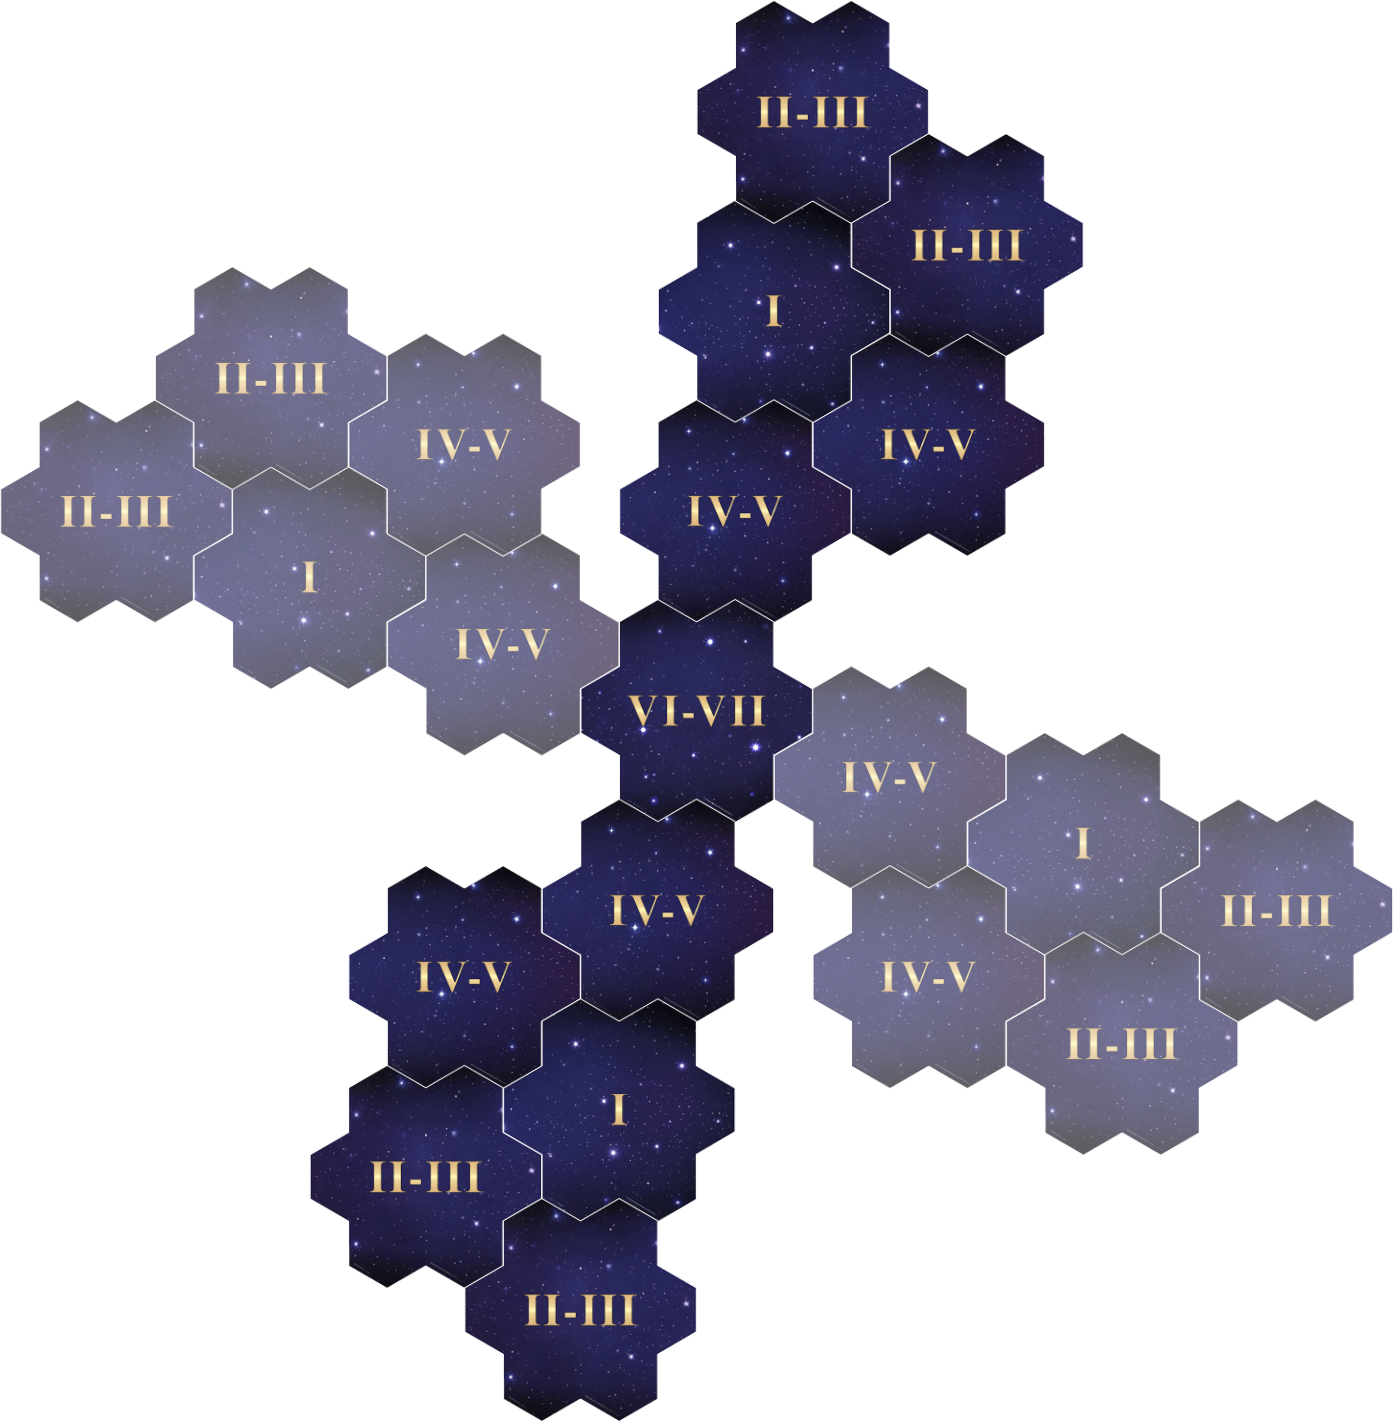
\includegraphics[width=1.0\linewidth]{\maps/trial_by_combat-2.4p.png}
  \captionof{figure}{\textbf{2/4-PLAYER SCENARIO}}
  \vfill
  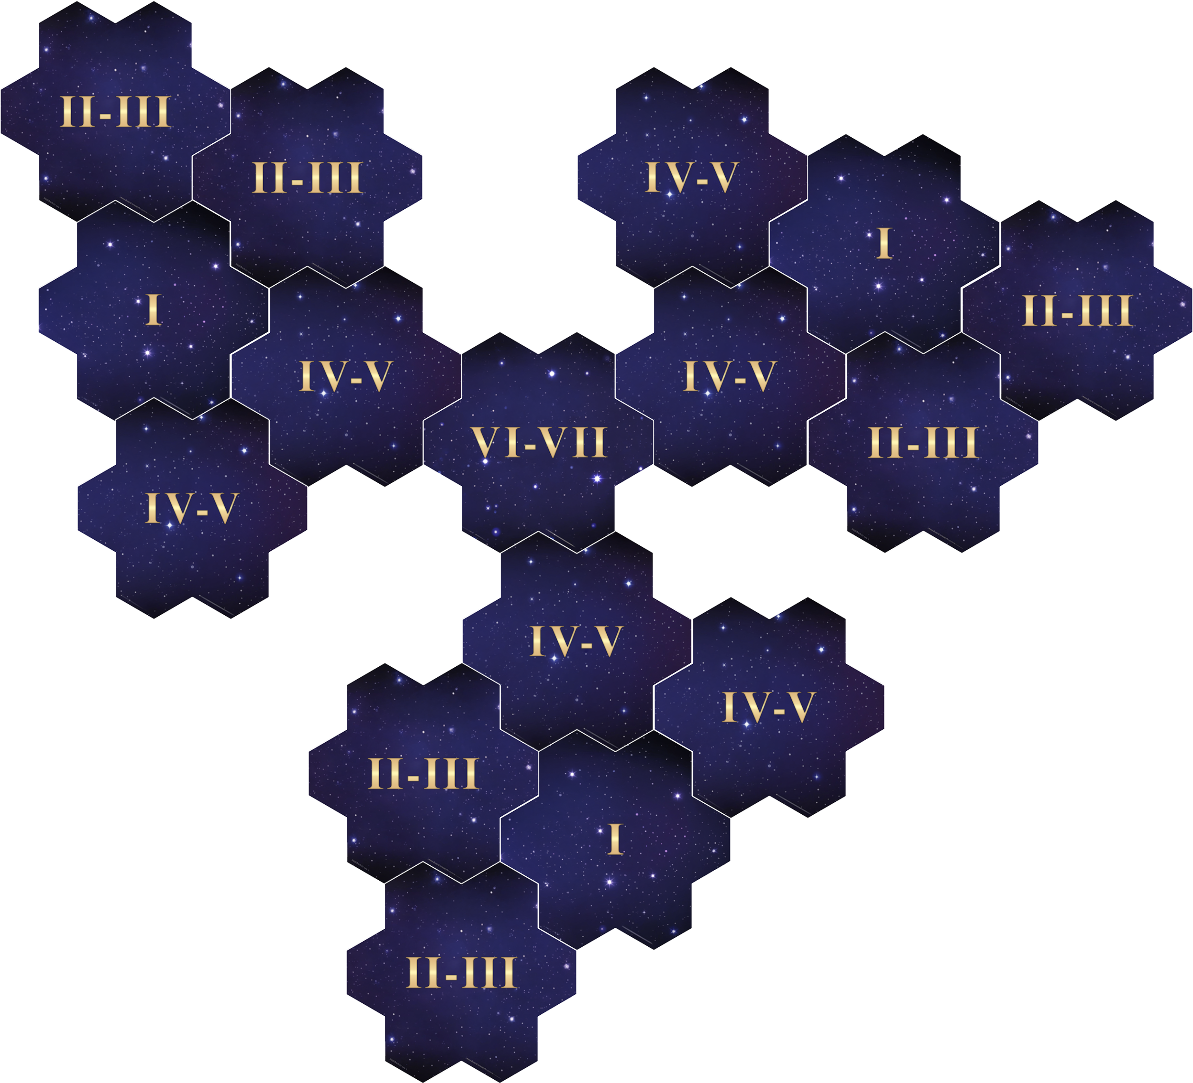
\includegraphics[width=1.0\linewidth]{\maps/trial_by_combat-3p.png}
  \captionof{figure}{\textbf{3-PLAYER SCENARIO}}
\end{center}

\end{multicols*}
